\documentclass[a4paper, 11pt]{article}
\usepackage{graphicx, float, url, hyperref, lscape, afterpage, amsthm, amsmath, mathtools, algorithmicx, algpseudocode}
\title{CS 210 Problem Set 1}
\author{Joshua Frankie Rayo\\ 2011-19612}
\date{\today}
\newtheorem{definition}{Definition}

\begin{document}
\maketitle

\section{Problem 1.2} 
Implement a merge sort that avoids defining a sentinel value.

\textbf{Solution.} We can implement the merging procedure to array C without sentinels by having iteration variables the two arrays A and B and taking note their position. This is given by the algorithm below:

\begin{algorithmic}
	\Function{Merge}{A, B}
	\State $C\gets []$
	\State $i\gets 0$
	\State $j\gets 0$
	\Repeat
	\If{$A[i] \leq B[j]$}
		\State $append(C, A[i])$
		\If{$i + 1 < length(A)$}
		\State $i \gets i+1$
		\EndIf
	\Else
		\State $append(C, B[j])$
		\If{$j + 1 < length(B)$}
		\State $j \gets j+1$
		\EndIf
	\EndIf
	\Until{$i+1=length(A) \And j+1=length(B)$}
	\EndFunction
\end{algorithmic}

\textbf{Example.} Consider merging two arrays:

\begin{center}
	\begin{tabular}{ c c c c c c }
		i & $\downarrow$\\
		\textbf{A} & 1 & 2 & 4 & 5\\
		j & $\downarrow$\\
		\textbf{B} & 2 & 3 & 6 & 8 & 9\\
		\textbf{C} \\
	\end{tabular}
\end{center}

\begin{center}
	\begin{tabular}{ c c c c c c }
		i & & $\downarrow$\\
		\textbf{A} & 1 & 2 & 4 & 5\\
		j & $\downarrow$\\
		\textbf{B} & 2 & 3 & 6 & 8 & 9\\
		\textbf{C} & 1\\
	\end{tabular}
\end{center}

\begin{center}
	\begin{tabular}{ c c c c c c }
		i & & & $\downarrow$\\
		\textbf{A} & 1 & 2 & 4 & 5\\
		j & $\downarrow$\\
		\textbf{B} & 2 & 3 & 6 & 8 & 9\\
		\textbf{C} & 1 & 2\\
	\end{tabular}
\end{center}

\begin{center}
	\begin{tabular}{ c c c c c c }
		i & & & $\downarrow$\\
		\textbf{A} & 1 & 2 & 4 & 5\\
		j & & $\downarrow$\\
		\textbf{B} & 2 & 3 & 6 & 8 & 9\\
		\textbf{C} & 1 & 2 & 2\\
	\end{tabular}
\end{center}

\begin{center}
	\begin{tabular}{ c c c c c c }
		i & & & $\downarrow$\\
		\textbf{A} & 1 & 2 & 4 & 5\\
		j & & & $\downarrow$\\
		\textbf{B} & 2 & 3 & 6 & 8 & 9\\
		\textbf{C} & 1 & 2 & 2 & 3\\
	\end{tabular}
\end{center}

\begin{center}
	\begin{tabular}{ c c c c c c }
		i & & & & $\downarrow$\\
		\textbf{A} & 1 & 2 & 4 & 5\\
		j & & & $\downarrow$\\
		\textbf{B} & 2 & 3 & 6 & 8 & 9\\
		\textbf{C} & 1 & 2 & 2 & 3 & 4\\
	\end{tabular}
\end{center}

\begin{center}
	\begin{tabular}{ c c c c c c c c}
		i & & & & $\downarrow$\\
		\textbf{A} & 1 & 2 & 4 & 5\\
		j & & & & $\downarrow$\\
		\textbf{B} & 2 & 3 & 6 & 8 & 9\\
		\textbf{C} & 1 & 2 & 2 & 3 & 4 & 5 & 6\\
	\end{tabular}
\end{center}

\begin{center}
	\begin{tabular}{c c c c c c c c c c}
		i & & & & $\downarrow$\\
		\textbf{A} & 1 & 2 & 4 & 5\\
		j & & & & & $\downarrow$\\
		\textbf{B} & 2 & 3 & 6 & 8 & 9\\
		\textbf{C} & 1 & 2 & 2 & 3 & 4 & 5 & 6 & 8 & 9\\
	\end{tabular}
\end{center}

Since $i$ and $j$ are both pointing to end of $A$ and $B$, the procedure will stop.

\section{Problem 1.3} Implement a merge sort that divides the array into three equal parts, sorts them, and does a three-way merge. Empirically compare its running time with standard merge sort.

\textbf{Solution.} The three-way merge sort is given by the following algorithm:

\begin{algorithmic}
	\Function{MergeSort3}{A}
	\State $n \gets length(A)$
	\If{$n \leq 1$}
		\Return A
	\EndIf
	\State $x \gets \lceil n/3 \rceil$
	\State $y \gets \lceil 2n/3 \rceil$
	\State \Return \Call{Merge3}{$A[0\ldots x-1], A[x \ldots y-1], A[y \ldots n-1]$}
	\EndFunction
\end{algorithmic}

\begin{algorithmic}
	\Function{Merge3}{$A_0, A_1, A_2$}
	\State \Return \Call{Merge}{$(A_0, Merge(A_1, A_2))$}
	\EndFunction
\end{algorithmic}

Comparing the running time with standard merge sort, we have

\begin{center}
	\begin{tabular}{c | c | c}
		N & 2-way & 3-way\\
		\hline
		1 & 0 & 0\\
		2 & 2 & 2.1031\\
		3 & 4.75489 & 5\\
		4 & 8 & 8.4124\\
		5 & 11.6096 & 12.2081\\
		6 & 15.5098 & 16.3093\\
		7 & 19.6515 & 20.6645\\
		8 & 24 & 25.2372\\
		9 & 28.5293 & 30\\
		10 & 33.2193 & 34.9317\\
	\end{tabular}
\end{center}

Comparing asymptotically as $N$ goes large, we have the following graph:

\begin{figure}[H]
	\centering
	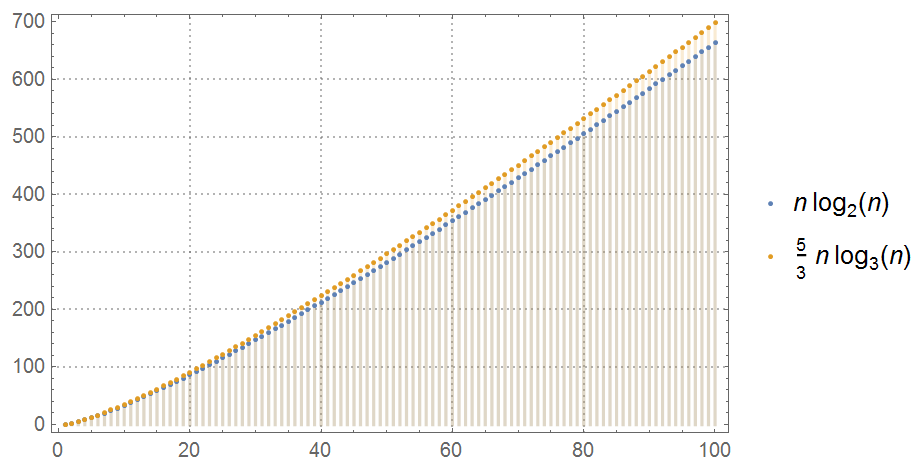
\includegraphics[width=\textwidth]{Capture}
\end{figure}

The 3-way merge sort generally takes more time than the 2-way merge sort.

\section{Problem 1.6} Analyze the number of compares used by the three-way merge sort.

\textbf{Solution.} The number of compares on the inner merging is $\frac{n}{3} + \frac{n}{3}$ and $\frac{n}{3} + \frac{2n}{3}$ for the outer merging. Then the total number of compares for the whole merging is $\frac{n + n + n + 2n}{3} = \frac{5n}{3}$. Given the three-way merge algorithm above, the total number of compares is given by
\begin{equation*}
C_n = 3C_{\lfloor n/3 \rfloor} + \frac{5n}{3}, \quad C_1 = 0.
\end{equation*}
Solving the recurrence relation in terms of $n = 3^m \geq 1$, we have:
\begin{align*}
C_{3^m} &= 3C_{3^{m-1}} + 5 \cdot 3^{m-1}\\
\frac{C_{3^m}}{3^m} &= \frac{C_{3^{m-1}}}{3^{m-1}} + \frac{5}{3}\\
\frac{C_{3^m}}{3^m} &= \frac{C_{3^{m-2}}}{3^{m-2}} + \frac{5}{3} + \frac{5}{3} = \frac{C_{3^0}}{3^0} + \frac{5m}{3} = \frac{5m}{3}\\
C_{3^m} &= \frac{5}{3}m \cdot 3^m\\
\Aboxed{
C_n &= \frac{5}{3}n \log_3(n)}
\end{align*}

\section{Problem 2.8} For \textit{f} linear, express the solution to the recurrence
\begin{equation*}
a_n = f(a_{n-1}, a_{n-2})
\end{equation*}
for $n>1$  in terms of $a_0, a_1, f(0, 0)$.

\textbf{Solution.} The solution is

\begin{equation*}
a_n = a_0 u_n + a_1 v_n + C*f(0,0)
\end{equation*}
where
\begin{equation*}
	u_n = f(u_{n-1}, u_{n-2})
\end{equation*}
for $n>1$ with $u_0=1$ and $u_1=0$.
and 
\begin{equation*}
v_n = f(v_{n-1}, u_{v-2})
\end{equation*}
for $n>1$ with $v_0=0$ and $v_0=1$ where $C$ is a constant obtained from the method of undetermined coefficients.

\textbf{Follow-up.} Find the solutions to
\begin{equation*}
a_n = f(a_{n-1}, a_{n-2}) - f(0, 0)
\end{equation*}
for $a_1=1, a_0=0$ and $a_0=1, a_1=0$.

\textbf{Solution.} This is a homogeneous linear recurrence.

\textbf{Case 1:} $a_1=1, a_0=0$. The solution is equal to

\begin{equation*}
v_n = f(v_{n-1}, v_{n-2})
\end{equation*}

where $v_0=0$ and $v_1=1$.

\textbf{Case 2:} $a_1=0, a_0=1$. The solution is equal to

\begin{equation*}
u_n = f(u_{n-1}, u_{n-2})
\end{equation*}

where $v_0=1$ and $v_1=0$.

\section{Problem 2.14} Write down the solution to
\begin{equation*}
a_n = x_n a_{n-1} + y_n
\end{equation*}
for $n>t$ in terms of the $x$'s, $y$'s and the initial value $a_t$.

\textbf{Solution.} Note that the summation factor is $x_n x_{n-1} x_{n-2} \ldots x_t$.
Divide both sides by summation factor and telescope until we get the closed form.

\begin{align*}
\frac{a_n}{x_n x_{n-1} \ldots x_t} &= \frac{a_{n-1}}{x_{n-1} x_{n-2} \ldots x_t} + \frac{y_n}{x_n x_{n-1} \ldots x_t}\\
&= \frac{a_{n-2}}{x_{n-2} x_{n-3} \ldots x_t} + \frac{y_{n-1}}{x_{n-1} x_{n-2} \ldots x_t} + \frac{y_n}{x_n x_{n-1} \ldots x_t}\\
&= \frac{a_{n-3}}{x_{n-3} x_{n-4} \ldots x_t} + \frac{y_{n-2}}{x_{n-2} x_{n-3} \ldots x_t} + \frac{y_{n-1}}{x_{n-1} x_{n-2} \ldots x_t} + \frac{y_n}{x_n x_{n-1} \ldots x_t}\\
\frac{a_n}{x_n x_{n-1} \ldots x_t}&= \frac{a_t}{x_t} + \frac{y_{t+1}}{x_{t+1} x_t} + \frac{y_{t+2}}{x_{t+2} x_{t+1} x_t} + \ldots + \frac{y_{n-1}}{x_{n-1} x_{n-2} \ldots x_t} + \frac{y_n}{x_n x_{n-1} \ldots x_t}\\
a_n &= a_t(x_{t+1} x_{t+2} \ldots x_n) + y_{t+1}(x_n x_{n-1} \ldots x_{t+2}) + y_{t+2}(x_n x_{n-1} \ldots x_{t+3})\\ &+ \ldots + y_{n-2}(x_n x_{n-1}) + y_{n-1} x_n + y_n\\
\Aboxed{a_n &= a_t \prod_{i=t+1}^{n} x_i + \sum_{i=t+1}^{n} \left[y_i \prod_{j=i+1}^{n} x_j\right]}
\end{align*}

\section{Problem 2.43.} Solve the recurrence
\begin{equation*}
a_n = \frac{\alpha a_{n-1} + \beta}{\gamma a_{n-1} + \delta}
\end{equation*}
for $n>0$ with $a_0=1$.

\textbf{Solution.} First, we guess the form of $a_n$ by getting $a_1, a_2$ and $a_3$.
\begin{align*}
a_0 &= 1\\
a_1 &= \frac{\alpha a_0 + \beta}{\gamma a_0 + \delta} = \frac{\alpha + \beta}{\gamma + \delta}\\
a_2 &= \frac{\alpha a_1 + \beta}{\gamma a_1 + \delta} = \frac{\alpha \left(\frac{\alpha + \beta}{\gamma + \delta}\right) + \beta}{\gamma \left(\frac{\alpha + \beta}{\gamma + \delta}\right) + \delta} = \frac{\alpha (\alpha + \beta) + \beta (\gamma + \delta)}{\gamma (\alpha + \beta) + \delta (\gamma + \beta)}\\
a_3 &= \frac{\alpha a_2 + \beta}{\gamma a_2 + \delta} = \frac{\alpha \left(\frac{\alpha (\alpha + \beta) + \beta (\gamma + \delta)}{\gamma (\alpha + \beta) + \delta (\gamma + \delta)}\right) + \beta}{\gamma \left(\frac{\alpha (\alpha + \beta) + \beta (\gamma + \delta)}{\gamma (\alpha + \beta) + \delta (\gamma + \delta)}\right) + \delta}\\ &= \frac{\alpha \left[\alpha (\alpha + \beta) + \beta (\gamma + \delta)\right] + \beta \left[\gamma (\alpha + \beta) + \delta (\gamma + \delta)\right]}{\gamma \left[\alpha (\alpha + \beta) + \beta (\gamma + \delta)\right] + \delta \left[\gamma (\alpha + \beta) + \delta (\gamma + \delta)\right]}
\end{align*}

Observing the pattern, we have the following system of linear homogeneous recurrence relations:
\begin{align*}
a_n &= \frac{b_n}{c_n}\\
b_n &= \alpha b_{n-1} + \beta c_{n-1}\\
c_n &= \gamma b_{n-1} + \delta c_{n-1}\\
b_0 &= 1\\
c_0 &= 1
\end{align*}

Solving for $b_n$ and $c_n$, we have
\begin{align*}
	\begin{bmatrix}
	b_n\\
	c_n
	\end{bmatrix}
	&=
	\begin{bmatrix}
	\alpha & \beta \\
	\gamma & \delta 
	\end{bmatrix}
	\begin{bmatrix}
	b_{n-1}\\
	c_{n-1}
	\end{bmatrix}\\
	\begin{bmatrix}
	b_n\\
	c_n
	\end{bmatrix}
	&=
	\begin{bmatrix}
	\alpha & \beta \\
	\gamma & \delta 
	\end{bmatrix}^2
	\begin{bmatrix}
	b_{n-2}\\
	c_{n-2}
	\end{bmatrix}\\
	\begin{bmatrix}
	b_n\\
	c_n
	\end{bmatrix}
	&=
	\begin{bmatrix}
	\alpha & \beta \\
	\gamma & \delta 
	\end{bmatrix}^n
	\begin{bmatrix}
	b_0\\
	c_0
	\end{bmatrix}
	=
	\begin{bmatrix}
	\alpha & \beta \\
	\gamma & \delta 
	\end{bmatrix}^n
	\begin{bmatrix}
	1\\1
	\end{bmatrix}
	=
	\mathbf{A}^n
	\begin{bmatrix}
	1\\1
	\end{bmatrix}
\end{align*}

To solve for the matrix power, we have $\mathbf{A}^n = PD^nP^{-1}$ where $P$ is the matrix of eigenvectors (as columns) of $A$ and $D$ is the diagonal matrix of eigenvalues. $\mathbf{A}$ has the following characteristic polynomial and corresponding eigensystem
\begin{align*}
	\lambda^2 &- (\alpha + \delta)\lambda + \alpha \delta - \beta \gamma = 0\\
	\lambda_{1, 2} &= \frac{1}{2}\left( \alpha + \delta \pm \Delta \right)\\
	v_{1, 2} &= \left[ -\frac{1}{2\gamma} \left(-\alpha + \delta \mp \Delta \right), 1 \right]^{\mathbf{T}}\\
	\Delta &= \sqrt{(\alpha - \delta)^2 + 4 \beta \gamma}
\end{align*}

\begin{landscape}
So the matrix power of $\mathbf{A}$ is
\begin{align*}
	\mathbf{A}^n &= PD^nP^{-1}\\
	\mathbf{A}^n &=
	\begin{bmatrix}
	-\frac{1}{2\gamma} \left(-\alpha + \delta - \Delta \right) & -\frac{1}{2\gamma} \left(-\alpha + \delta + \Delta \right)\\
	1 & 1
	\end{bmatrix}
	\begin{bmatrix}
	\frac{1}{2}\left( \alpha + \delta + \Delta \right) & 0 \\
	0 & \frac{1}{2}\left( \alpha + \delta - \Delta \right)
	\end{bmatrix}^n
	\begin{bmatrix}
	-\frac{\gamma }{\Delta} & \frac{\alpha -\delta + \Delta}{2 \Delta}\\
	\frac{\gamma }{\Delta} & \frac{-\alpha +\delta -\Delta}{2 \Delta}
	\end{bmatrix}
\end{align*}

\begin{align*}
\mathbf{A}^n &= 
\begin{bmatrix}
\frac{2^{-n-1} \left(\left(\Delta-\alpha +\delta \right) \left(-\Delta+\alpha +\delta \right)^n+\left(\Delta+\alpha -\delta \right) \left(\Delta+\alpha +\delta \right)^n\right)}{\Delta} & \frac{\beta  2^{-n} \left(\left(\Delta+\alpha +\delta \right)^n-\left(-\Delta+\alpha +\delta \right)^n\right)}{\Delta}\\
\frac{\gamma  2^{-n} \left(\left(\Delta+\alpha +\delta \right)^n-\left(-\Delta+\alpha +\delta \right)^n\right)}{\Delta} & \frac{2^{-n-1} \left(\left(\Delta+\alpha -\delta \right) \left(-\Delta+\alpha +\delta \right)^n+\left(\Delta-\alpha +\delta \right) \left(\Delta+\alpha +\delta \right)^n\right)}{\Delta}
\end{bmatrix}\\
\mathbf{A}^n
\begin{bmatrix}
1\\1
\end{bmatrix}
&=
\begin{bmatrix}
\frac{\left((-\alpha -2 \beta +\delta ) \left(-\Delta+\alpha +\delta \right)^n+\Delta \left(-\Delta+\alpha +\delta \right)^n+(\alpha +2 \beta -\delta ) \left(\Delta+\alpha +\delta \right)^n+\Delta \left(\Delta+\alpha +\delta \right)^n\right)}{\Delta 2^{n+1} }
\\
\frac{\left((\alpha -2 \gamma -\delta ) \left(-\Delta+\alpha +\delta \right)^n+\Delta \left(-\Delta+\alpha +\delta \right)^n+(-\alpha +2 \gamma +\delta ) \left(\Delta+\alpha +\delta \right)^n+\Delta \left(\Delta+\alpha +\delta \right)^n\right)}{\Delta 2^{n+1}}
\end{bmatrix} = 
\begin{bmatrix}
b_n\\c_n
\end{bmatrix}
\end{align*}

Therefore, the solution is
\begin{align*}
\Aboxed{
a_n = \frac{(-\alpha -2 \beta +\delta ) \left(-\Delta+\alpha +\delta \right)^n+\Delta \left(-\Delta+\alpha +\delta \right)^n+(\alpha +2 \beta -\delta ) \left(\Delta+\alpha +\delta \right)^n+\Delta \left(\Delta+\alpha +\delta \right)^n}{(\alpha -2 \gamma -\delta ) \left(-\Delta+\alpha +\delta \right)^n+\Delta \left(-\Delta+\alpha +\delta \right)^n+(-\alpha +2 \gamma +\delta ) \left(\Delta+\alpha +\delta \right)^n+\Delta \left(\Delta+\alpha +\delta \right)^n}}
\end{align*}

where $\Delta = \sqrt{(\alpha - \delta)^2 + 4 \beta \gamma}$.

\end{landscape}
\end{document}